\section{Dart applications}

Creating a Flutter application can be done easily through the command line interface. 
To initiate a new application, use the following command:
\begin{verbatim}
    flutter create app_name
\end{verbatim}
This command generates a directory structure containing various subdirectories and files. 
Some of these subdirectories contain auto-generated code for different platforms, while others are critical for development:
\begin{itemize}
    \item \texttt{lib} directory: this folder holds all the handwritten code for your application.
    \item \texttt{pubspec.yaml} file: this file serves as the application's table of contents. 
        It is used to import external libraries and declare dependencies.
\end{itemize}
To run the application, execute the command:
\begin{verbatim}
    flutter run
\end{verbatim}
This command allows you to choose the platform on which you want to run the application. 
If certain platforms are unavailable on your development device, Flutter will emulate the desired device. 

Initially, the \texttt{lib} directory contains a file named \texttt{main.dart}, which includes the following code:
\begin{verbatim}
import 'package:flutter/material.dart';
    
void main() {
    runApp();
}
\end{verbatim}
Depending on the desired look and feel, you can import either \texttt{material.dart} for Material Design or \texttt{cupertino.dart} for iOS-style components. 
The \texttt{main} function contains the \texttt{runApp} method, which initializes the application.

The \texttt{runApp} function takes a given Widget and sets it as the root of the widget tree. 
This tree typically consists of two widgets: the Center widget and its child, the Text widget.
The Flutter framework ensures that the root widget covers the entire screen.

\subsection{Functions}
In Dart, a function can have any number of required positional parameters, which may be followed by either named parameters or optional positional parameters, but not both simultaneously. 
Named parameters are optional unless explicitly marked as required. 
You can also define default values for both named and positional parameters using the equals sign (=). 
These default values must be compile-time constants, and if no default value is provided, it defaults to null.

\subsection{Commas}
It is a best practice to always add a trailing comma at the end of a parameter list—this applies to functions, methods, and constructors where maintaining formatting is important. 
Adding trailing commas helps the automatic formatter insert the appropriate amount of line breaks, ensuring your code adheres to Flutter's styling guidelines.

\subsection{Widgets}
The structure of a Flutter application is fundamentally composed of widgets, which are the building blocks of the user interface. 
The following figure illustrates the material design structure used in Flutter applications:
\begin{figure}[H]
    \centering
    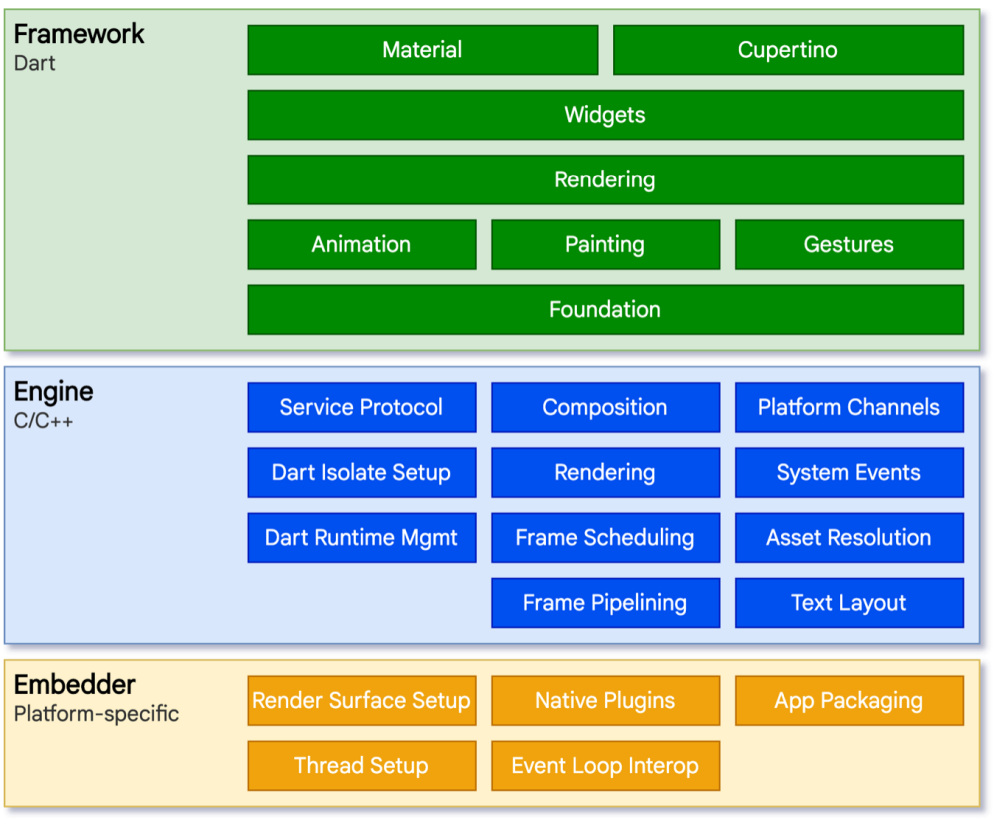
\includegraphics[width=0.75\linewidth]{images/flutter.png}
    \caption{Material structure}
\end{figure}
In Flutter, graphical user interfaces (GUIs) are created entirely through code, where nearly everything is represented as a widget. 
Key characteristics of widgets include:
\begin{itemize}
    \item \textit{Immutability}: a widget is an immutable object, meaning that once it is created, its properties cannot be changed. 
        Instead, to modify a widget's appearance or behavior, a new widget must be created.
    \item \textit{Composability}: widgets are composable, allowing developers to combine existing widgets to build more complex interfaces. 
        This enables the creation of new widgets by composing smaller, reusable ones.
    \item \textit{Descriptive nature}: widgets describe what the GUI should look like. 
        They provide a visual representation of the interface and its components.
\end{itemize}
When the state of a widget changes, the Flutter framework responds by rebuilding the affected widget. 
The framework performs the following steps:
\begin{enumerate}
    \item \textit{Diff computation}: it computes the difference between the current widget state and the previous rendering, determining what has changed.
    \item \textit{Minimal changes}: the framework identifies the minimal set of changes needed to update the interface, optimizing performance.
    \item \textit{Selective re-rendering}: only the parts of the UI that have changed are re-rendered, which enhances efficiency and responsiveness.
\end{enumerate}
This architecture of widgets allows for flexible and dynamic user interfaces that can easily adapt to user interactions and data changes.